\documentclass{subfiles}

\begin{document}

    \chapter{Introducción}
    \label{chap:1}

        \section{Introducción}
        \label{sec:introduccion}

        {El \TFG supone el último paso para obtener la titulación cursada, y se muestra de manera muy intimidante al alumno. Por mucho que otros compañeros de años anteriores intenten suavizar su dificultad o la necesidad de hacer algo grande, uno no deja de verlo como la culminación de varios años de aprendizaje en un estudio superior. Por eso, fue difícil elegir algo que realizar.}
      
        \paragraph{}
        {Durante varios años, estuve dispuesto a llevar mi propio proyecto con varias ideas que fui reservando para más adelante, e incluso fueron varias las revisiones que hice a las ideas preparadas para distintos trabajos por distintos profesores. Sin embargo, a medida que se iba acercando la fecha de comenzar este proyecto, iba creciendo la necesidad de comenzar a trabajar y tener mis propios ingresos. Así, y teniendo el \TFG en mente, comencé a buscar empleo planteando a las empresas que me concedían entrevista dos condiciones: media jornada para poder terminar mis estudios y que me ofrecieran un proyecto válido para un \tfg para poder terminar mi carrera.}
      
        \paragraph{}
        {Fue así como entré en \silverstorm, ahora \thirdera, después de su adquisición por parte de esta última. Ellos me concedieron la flexibilidad necesaria para compaginar empleo y estudios, así como facilidades a la hora de realizar los exámenes de la Universidad. Además, al entrar en el equipo de innovación, sabía que me podrían ofrecer un proyecto que se distinguiese de los que ofrecían al resto de estudiantes que trabajaban en la empresa.}

        \paragraph{}
        {\thirdera, al igual que \silverstorm en su momento, es una empresa dedicada a la digitalización y automatización de procesos a través de la herramienta \servicenow, en la que está especializada. El trabajo con esta herramienta consiste en ayudar a sus clientes a implantarla y adaptarla al uso que necesiten de la misma, de manera que el impacto para los usuarios sea el mínimo y la optimización de procesos  de negocio se amplíe paulatinamente. Por otro lado, \servicenow permite también la creación de plugins que pueden ser lanzadas al mercado.}

        \section{Motivación}
        \label{sec:motivacion}
        
        \paragraph{}
        {Tras un tiempo, y después de comentarles que quería comenzar a desarrollar mi \TFG, me ofrecieron el proyecto que se explicará en esta memoria. Por aquel entonces, la página web de \silverstorm desarrollada en \wordpress contaba con un estilo sencillo y familiar para que los usuarios que entrasen conociesen la empresa y pudieran obtener la información que desearan de ella: a qué nos dedicamos, cómo y con qué trabajamos, qué clientes tenemos o hemos tenido, de qué ofertas de trabajo disponemos, etc. No obstante, esta no lograba destacar sobre otras webs corporativas: sus animaciones eran aquellas que ofrecía \wordpress, los dibujos utilizados eran de una colección de imágenes de stock retocadas y su sencillez implicaba una cierta monotonía.}
        
        \paragraph{}
        {La idea del proyecto era añadir un pequeño detalle a esta página que hiciera que esta destacara un poco más. La propuesta consistía en generar un pequeño avatar que pudiese contar, en cada una de las secciones, lo que el usuario podía encontrar. Este avatar aparecería en el plano real mediante \ra, una tecnología en pleno auge \cite{Xiong2021} que reforzaría la idea de que la empresa se mantiene en contacto con las últimas tendencias tecnológicas. Además, para facilitar el uso de la cámara para ofrecer imágenes del mundo real, era imprescindible que el usuario accediese a esta experiencia a través del móvil.}

        \section{Objetivos}
        \label{sec:objetivos}
        {El objetivo general consiste en montar una aplicación web de \ra capaz de mostrar modelos tridimensionales con animación y sonido sincronizados en el entorno real del usuario. Esta aplicación debe ser soportada en los dispositivos móviles actuales. Para conseguir esto, los objetivos se desglosaron en varios puntos.}

        \paragraph{}
        {Debido a que el trabajo con estas tecnologías era nuevo para nuestro equipo y carecíamos de experiencia al respecto, el primer punto a abordar fue la \textbf{investigación} sobre estas tecnologías. En primer lugar, se tomaron como referencia algunas aplicaciones publicitarias que utilizaban unas versiones algo más rudimentarias de \ra donde, escaneando un código QR, aparecía en pantalla una persona comentando promociones sobre la imagen grabada por la cámara del móvil. Nuestra intención era investigar qué tecnología se usó en ese caso o en otros casos donde el resultado fuese mejor que el de partida.}
        
        \paragraph{}
        {Por supuesto, y dado que el proyecto mayoritariamente trabajaría sobre la tecnología utilizada, el siguiente objetivo sería aprender a utilizarla y \textbf{generar una estructura eficaz} y escalable que permitiese futuras mejoras.}

        \paragraph{}
        {Para complementar la experiencia inmersiva de la aplicación, se añadiría \textbf{sonido espacial} al mismo sistema. Esto permitiría que un usuario con auriculares pudiera reconocer, sin mirar a la pantalla, la dirección de la que procedía el sonido y la distancia que le separaba del origen de este.}
        
        \paragraph{}
        {También tendríamos que \textbf{desarrollar un modelo en 3D} que funcionase como nuestro avatar. Para ello, habría que buscar herramientas de creación, diseño y modelado en 3D, además de aprender a utilizarlos para obtener un resultado satisfactorio.}
        
        \paragraph{}
        {Para que diese la impresión de que el modelo fuese el que dijera todo lo mencionado en la grabación, sería necesario \textbf{sincronizar la voz con los gestos faciales} y los labios del modelo. Para esta <<sincronización labial>>, sería más eficiente buscar una aplicación o herramienta que fuese fácil de configurar e hiciese gran parte del trabajo. Por lo tanto, este objetivo se podría dividir en buscar una herramienta de sincronización labial, aprender a utilizarla y desplegar su funcionalidad sobre el proyecto.}
        
        \paragraph{}
        {Sería necesario también \textbf{generar una animación} para el resto del cuerpo del modelo 3D, de manera que este no resultara demasiado estático al hablar y diese una impresión algo más realista.}
        
        \paragraph{}
        {El sistema tiene que ser \textbf{accesible a través de la web}, por lo que sería necesario también alojarlo en un servidor que almacenase toda la funcionalidad, así como los protocolos necesarios para que la conexión fuese fiable y segura.}

        \paragraph{}
        {A mayores, otro punto a analizar en el proyecto era la accesibilidad del usuario a esta aplicación. Debido a la finalidad de la web, con obvias intenciones comerciales y laborales, el equipo encargado de desarrollar originalmente esta consideró que la mayor parte de los usuarios que visitaban la página accedían desde ordenadores, siendo una menor proporción los usuarios que accedían desde móviles o tablets. Por esta razón, se consideró que la mejor forma de hacer que un usuario pasara de un ordenador a un móvil era introduciendo un código \textbf{QR que enlazase directamente a este sistema}. En caso de que el usuario navegase desde el móvil, el mismo código funcionaría a la vez como un botón con la capacidad de redirigir.}


        \section{Conceptos de Realidad Aumentada}
        \label{sec:conceptos_de_realidad_aumentada}

        Antes de comenzar a explicar en qué consiste este proyecto, es importante fijar algunos conceptos de \ra tal y como se van a utilizar en este tema, de manera que no queden ambigüedades a partir de este punto.

        \subsection{Realidad}
        \label{sec:realidad}
        El concepto más importante y a la vez básico a dejar claro es el concepto de \realidad. Para nuestro sistema, se considera \realidad al conjunto de objetos, información y estímulos, principalmente visuales, que componen nuestro entorno y que percibimos a través de nuestros sentidos. Así, si nos encontrásemos en nuestra casa, podríamos percibir varios elementos a través de la \realidad: una televisión, un sofá, una temperatura cálida, una iluminación baja, el ruido de un ventilador...

        \subsection[Realidad Aumentada y Realidad Virtual]{Realidad Aumentada y Realidad Virtual}
        \label{sec:realidad_aumentada_y_realidad_virtual}

        La \ra y la \rv son dos conceptos que a menudo se confunden por ser relativamente nuevos y por sus puntos en común. Sin embargo, los resultados pueden llegar a ser muy distintos o incluso opuestos en algunos casos. En ambos existe información generada a través de sistemas informáticos, pero las diferencias son ampliamente notables \cite{web:diferencias_ra_rv}.

        \begin{figure}[H]
        \centering
        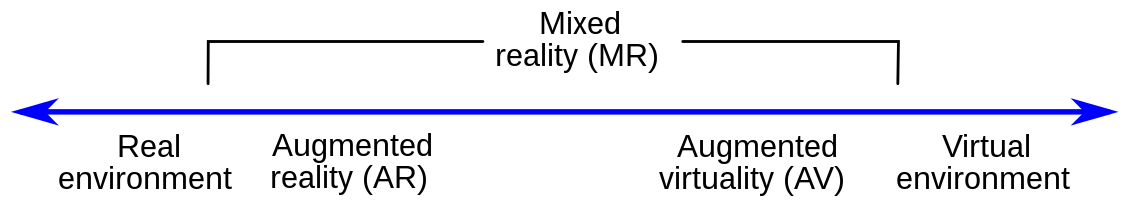
\includegraphics[width=0.8\textwidth]{reality_continuum}
        \caption{Espectro entre un entorno real y un entorno virtual. Fuente: \citetitle{web:wikipedia_realidad_aumentada}}
        \label{fig:reality_continuum}
        \end{figure}

        \paragraph{}
        La diferencia más destacable es el concepto de \realidad anteriormente mencionado, así como su uso: en la \rv, todos los elementos son generados digitalmente, de manera que la \realidad percibida es totalmente distinta a nuestro entorno <<real>>. Para esto, comúnmente se hace uso de las gafas de \rv, que aíslan la visión del usuario para que solo pueda captar la información generada y transmitida por las gafas.
    
        \paragraph{}
        Sin embargo, en el caso de la \ra, la intención es ampliar en tiempo real los datos captados de la \realidad, por lo que la base en estas tecnologías siempre serán imágenes e información de nuestro entorno. A esto se le debe sumar todo aquello que añada el sistema para <<ampliar>> la \realidad: figuras, texto, imágenes, etc. Estas últimas se encontrarán superpuestas sobre lo captado del entorno de manera fidedigna y que ofrezca más valor a lo naturalmente captado.

        \begin{figure}
        \centering
        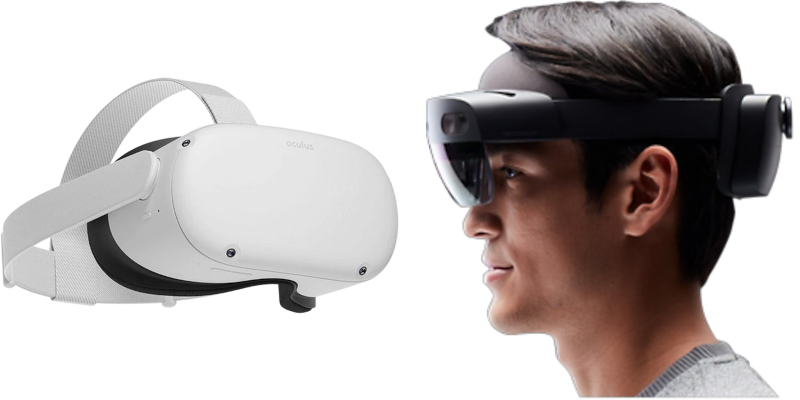
\includegraphics[width=0.8\textwidth]{vr_ar_devices}
        \caption{A la izquierda, las Meta Quest 2, las gafas de \rv de Meta. A la derecha, las Microsoft Hololens, las gafas de \ra de Microsoft. Fuentes: \citetitle{web:meta_quest2} y \citetitle{web:microsoft_hololens}}
        \label{fig:vr_ar_devices}
        \end{figure}
    
        \paragraph{}
        Otra gran diferencia se puede encontrar en los dispositivos utilizados para aplicar ambas tecnologías. Como se comentó antes, la \rv utiliza unas gafas que aíslan al usuario de la \realidad. Cabe mencionar también que estas gafas son de uso exclusivo para dicha tecnología, así como su elevado coste, ya que son una tecnología que, pese a que ya lleva varios años de desarrollo y mejora, aún necesita asentarse correctamente en el mercado. La \ra, en cambio, se apoya generalmente en dos tecnologías dependiendo de su uso: por un lado, para los usos más cotidianos (aunque a veces también se encuentran en este grupo usos profesionales), se suele implementar en dispositivos móviles, donde la cámara capta las imágenes del entorno y el propio dispositivo móvil añade la información pertinente; por otro lado, y para usos exclusivamente profesionales, muchas empresas han comenzado a utilizar gafas de \ra donde, mediante un juego de espejos, el usuario es capaz de ver información añadida a su entorno.

        \paragraph{}
        Por último, pese a que ya se ha adelantado este punto previamente, por lo menos hasta el día de hoy la \rv se está especializando más en el área lúdica, al ser los desarrolladores de videojuegos los principales interesados en esta tecnología, aunque no se descarta que en el futuro pueda aplicarse para motivos más profesionales. La \ra también se utiliza para este fin, pero ha conseguido entrar en el área profesional como herramienta para varios sectores, como es el del marketing, donde aplicaciones como la de Ikea \cite{web:ikea_placeapp} permiten al usuario colocar muebles de la tienda en su propia casa para probarlos y, así, impulsar las ventas.

        \subsection{Sonido espacial}
        \label{sec:introduccion_sonido_espacial}
        Para ampliar la sensación de que los elementos que añadamos mediante nuestra aplicación forman parte de nuestro entorno, las voces de los asistentes virtuales dispondrán de una propiedad denominada sonido espacial, que es la propiedad por la cual somos capaces de identificar la posición, orientación y distancia del origen de un sonido \cite{web:wikipedia_localizacion_sonido}.

        \paragraph{}
        Utilizando como ejemplo el sonido emitido por nuestra televisión. Si cerráramos los ojos, seríamos capaces de interpretar varios datos únicamente por el sonido: no solo de dónde procede o a cuánta distancia está, sino que también podríamos percibir información de nuestro entorno según el eco que produce, como por ejemplo si estamos en una habitación o al aire libre o el tamaño de la habitación en el primer caso.

        \paragraph{}
        Toda esta información se percibe gracias a cómo el cerebro interpreta los fenómenos físicos a través de los cuáles se transmite el sonido \cite{web:resonance_audio_localizacion_sonido, web:wikipedia_localizacion_sonido}. Por ejemplo, somos capaces de interpretar si un sonido viene desde nuestra derecha o desde nuestra izquierda a través de la \textit{diferencia de tiempo interaural}: si un sonido tarda más en llegar a nuestro oído derecho que a nuestro oído izquierdo, quiere decir que el sonido procede de nuestra izquierda. Además, la diferencia de tiempo entre ambos oídos nos indicará también si el sonido está totalmente a nuestra izquierda o, en cambio, está situado en un ángulo distinto.

        \begin{figure}
        \centering
        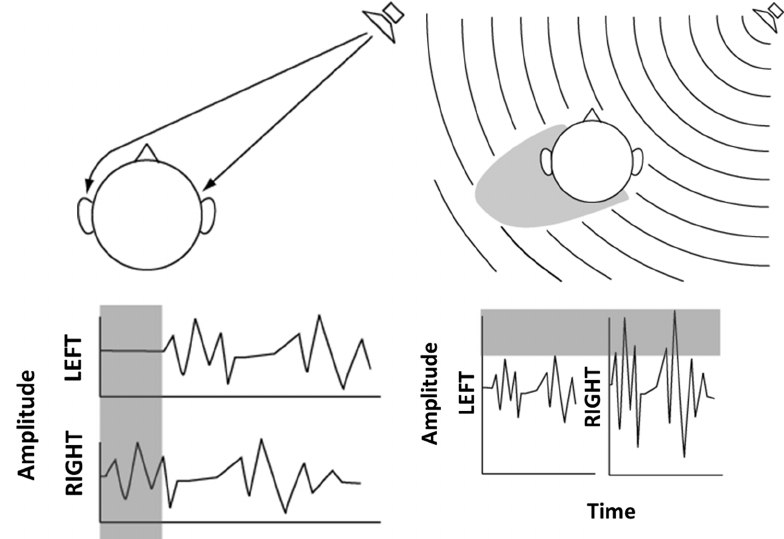
\includegraphics[width=0.8\textwidth]{img/ITD_ILD.png}
        \caption{A la izquierda, una representación de la diferencia de tiempo interaural. A la derecha, una representación de la diferencia de nivel interaural. Fuente: \citetitle{art:mroz_spatialaudio}.}
        \label{fig:ITD_ILD}
        \end{figure}

        \paragraph{}
        Otra forma que tiene nuestro cerebro de detectar la posición de un sonido es utilizando los cambios sutiles que se generan en las altas frecuencias cuando las ondas son interceptadas por la forma de nuestra oreja o de nuestra cabeza, conocidos como \textit{diferencia de nivel interaural}. Por ejemplo, un ruido no nos llegará de la misma manera si se origina delante de nosotros o detrás de nosotros. En el primer caso, el sonido será parcialmente tapado por el trago de la oreja. Pero en el segundo caso, el sonido será interceptado por gran parte del pabellón auricular. En el segundo caso, las frecuencias más altas pueden llegar a perderse, por lo que nuestro cerebro interpretaría que el origen del ruido se ha producido detrás de nosotros, mientras que en el primer caso, al mantenerse más altas frecuencias, interpretaríamos que la posición se genera delante de nosotros. Esto, en combinación con la inferencia anteriormente comentada, nos permitiría ubicar un sonido en el plano horizontal.

        \paragraph{}
        Por último, cabe mencionar que estas técnicas usadas por nuestro cerebro para ubicar sonidos en el plano horizontal son muy similares a las que utiliza para ubicarlos en el vertical o incluso para determinar la distancia a la que está dicho sonido, ya esté estático o en movimiento.
        
        \section{Tecnologías utilizadas}
        \label{sec:tecnologias_utilizadas}

        Para elaborar nuestra aplicación de \ra, nos hemos apoyado principalmente en tres herramientas ya existentes, cuyo uso se explicará con detalle más adelante.

        \paragraph{}
        El primero y más importante es \webxr \cite{web:webxr}. Esta es una interfaz para generar entornos tanto de \ra como de \rv y que facilita al desarrollador la interacción con el hardware. Aunque su uso se preparó para generar estos entornos en dispositivos de \rv exclusivamente, más tarde se actualizó para poder ser utilizado en el navegador \googlechrome (versión 79) para móviles \android. Gracias a \webxr, podremos acceder a aspectos básicos para esta tecnología, como el acceso a la cámara del dispositivo, la ubicación y orientación del mismo, la creación de una sesión interactiva...

        \paragraph{}
        Para poder modificar y manipular los modelos en 3D que comentaremos en el desarrollo de esta memoria, hemos recurrido a la librería \threejs \cite{web:threejs}, una librería centrada en la generación de modelos y gráficos 3D para navegadores web para \js. Esta puede utilizar varios formatos de modelos 3D como FBX, Collada o OBJ, pero la documentación recomienda encarecidamente utilizar el formato \gltf por estar más centrado en su uso en tiempo de ejecución: es un formato muy compacto y rápido de cargar. \webxr se apoya en esta librería para mostrar estos modelos en imágenes del mundo real (\ra) o en entornos totalmente generados (\rv).

        \paragraph{}
        La última librería utilizada es \resonanceaudio \cite{web:resonance_audio}, la cual permite ampliar las funcionalidades básicas de sonidos que contiene HTML en conjunto con \js. En concreto, \resonanceaudio permite simular sonidos espaciales recreando las características que permiten a nuestro cerebro posicionar un sonido a nuestro alrededor. Además, dispone de personalizaciones para el sonido emitido, como la simulación de eco en interiores dependiendo de los materiales de las paredes, techo y suelo que rodeen al foco del sonido.
        
\end{document}
